    \documentclass[11pt,a4paper,oneside]{report}
    \usepackage[utf8]{inputenc}
    \usepackage[T1]{fontenc}
    \usepackage[french]{babel}
    \usepackage{graphicx}
    \usepackage{hyperref}
    \usepackage{geometry}
    \usepackage{xcolor}
    \usepackage{listings}
    \usepackage{float}
    \usepackage{booktabs}
    \usepackage{amsmath}
    \usepackage{amsfonts}
    \usepackage{setspace}
    \usepackage{titlesec}
    \usepackage{fancyhdr}
    \usepackage{tcolorbox}
    \usepackage{enumitem}
    \usepackage{longtable}

    \geometry{top=2.5cm, bottom=2.5cm, left=3cm, right=2.5cm}
    \onehalfspacing

    % --- Configuration des couleurs ---
    \definecolor{mainblue}{RGB}{0,71,171}
    \definecolor{codegreen}{rgb}{0,0.6,0}
    \definecolor{codegray}{rgb}{0.5,0.5,0.5}
    \definecolor{codepurple}{rgb}{0.58,0,0.82}
    \definecolor{backcolour}{rgb}{0.98,0.98,0.96}

    % --- Configuration des listings ---
    \lstset{
        language=Python,
        backgroundcolor=\color{backcolour},
        commentstyle=\color{codegreen},
        keywordstyle=\color{mainblue}\bfseries,
        numberstyle=\tiny\color{codegray},
        stringstyle=\color{codepurple},
        basicstyle=\ttfamily\scriptsize,
        breakatwhitespace=false,
        breaklines=true,
        captionpos=b,
        keepspaces=true,
        numbers=left,
        numbersep=5pt,
        showspaces=false,
        showstringspaces=false,
        showtabs=false,
        tabsize=2,
        frame=single,
        rulecolor=\color{codegray}
    }

    % --- Header & Footer ---
    \pagestyle{fancy}
    \fancyhf{}
    \fancyhead[L]{\small Smart Shoe Intelligence Project}
    \fancyhead[R]{\small Rapport Académique de Fin de Module}
    \fancyfoot[C]{\thepage}

    % --- Redéfinition des titres ---
    \titleformat{\chapter}[display]
    {\normalfont\bfseries\color{mainblue}}
    {\filleft\Large\chapternameline \Huge\thechapter}
    {1ex}
    {\titlerule\vspace{1ex}\filright}
    \newcommand{\chapternameline}{Chapitre }

    % -----------------------------------------------------------------------------
    % DOCUMENT START
    % -----------------------------------------------------------------------------
    \begin{document}

    % --- PAGE DE GARDE ---
    \begin{titlepage}
    \thispagestyle{empty}
    \begin{center}

    \begin{minipage}[c]{0.25\textwidth}
    \centering
    \includegraphics[width=1.0\linewidth,keepaspectratio]{lg.png}
    \end{minipage}
    \hfill
    \begin{minipage}[c]{0.25\textwidth}
    \centering
    \includegraphics[width=1.0\linewidth,keepaspectratio]{image.png}
    \end{minipage}

    \vspace{1.8cm}

    {\Large \textbf{Faculté des Sciences et Techniques de Tanger}}\\[0.3cm]
    {\large \textbf{Département Génie Informatique}}\\[0.3cm]
    {\large \textbf{Cycle d’ingénieur Logiciels et Systèmes Intelligents -- S3}}\\[0.3cm]

    \rule{\linewidth}{0.7pt}\\[0.8cm]
    {\LARGE \textbf{Smart Shoe Intelligence Pipeline}}\\[0.2cm]
    \rule{\linewidth}{0.7pt}\\[2.5cm]

    {\Large \textbf{Rapport de Projet de Fin de Module}}\\[2.5cm]

    \setlength{\parindent}{0pt}
    \begin{minipage}[t]{0.48\textwidth}
    \raggedright
    \textbf{Étudiants :}\\
    MOHAND OMAR Moussa \\
    ESSALHI Salma
    \end{minipage}
    \hfill
    \begin{minipage}[t]{0.48\textwidth}
    \raggedleft
    \textbf{Professeur :}\\
    Abdelhadi FENNAN
    \end{minipage}

    \vspace{1.2cm}

    \textbf{Année universitaire :} 2025--2026

    \vfill

    \end{center}
    \end{titlepage}

    \pagenumbering{roman}
    \tableofcontents
    \newpage

    % --- GLOSSAIRE ---
    \chapter*{Glossaire Technique Détaillé}
    \addcontentsline{toc}{chapter}{Glossaire Technique Détaillé}
    \begin{description}
        \item[A2A (Agent-to-Agent)] : Architecture logicielle où des unités autonomes (agents) collaborent pour exécuter un workflow complexe sans intervention humaine directe.
        \item[API (Application Programming Interface)] : Interface logicielle permettant à deux applications de communiquer entre elles, utilisée ici pour interroger Gemini et Groq.
        \item[Clustering] : Technique d'apprentissage non supervisé visant à diviser une population en groupes homogènes (les clusters).
        \item[Database Schema] : Structure logique qui définit la manière dont les données sont organisées dans une base de données MySQL.
        \item[Feature Engineering] : Processus de transformation de données brutes en variables (features) exploitables par un modèle de Machine Learning.
        \item[Hyperparamètre] : Paramètre dont la valeur est fixée avant le lancement du processus d'apprentissage du modèle (ex: max\_depth dans XGBoost).
        \item[JSON (JavaScript Object Notation)] : Format de donnée léger utilisé pour l'échange de données entre le serveur (boutique Shopify) et le client (scraper).
        \item[LLM (Large Language Model)] : Réseau de neurones profond entraîné sur du texte pour comprendre et générer du langage humain.
        \item[Pipeline] : Suite d'étapes automatisées de traitement de données où la sortie d'une étape sert d'entrée à la suivante.
        \item[Regex (Regular Expression)] : Séquence de caractères formant un modèle de recherche pour la manipulation de chaînes de caractères.
        \item[Thread-safe] : Qualité d'un code ou d'une structure de données pouvant être accédé simultanément par plusieurs threads sans provoquer de corruption.
    \end{description}

    \newpage
    \pagenumbering{arabic}

    % -----------------------------------------------------------------------------
    \chapter{Introduction et Problématique Stratégique}
    % -----------------------------------------------------------------------------
    \section{L'Émergence du E-Commerce Intelligent}
    L'industrie mondiale de la chaussure est passée d'un modèle traditionnel à une ère axée sur les données. La personnalisation et la réactivité du marché exigent une analyse granulaire des stocks et des tendances.

    \section{Défis du Web Scraping de Nouvelle Génération}
    Le scraping classique, fondé sur des règles statiques, échoue face à la complexité des sites modernes. Le défi majeur est l'extraction de la \textbf{sémantique} : comprendre si un produit est réellement pertinent par rapport à une niche spécifique.

    \section{Innovation de Smart Shoe Intelligence}
    Notre projet propose une architecture en 6 phases où chaque phase est vérifiée par une instance de \textbf{Reasoning AI}. Le but n'est pas seulement de collecter massivement, mais de collecter \textbf{intelligemment}.

    % -----------------------------------------------------------------------------
    \chapter{Architecture de Système et Flux de Travail}
    % -----------------------------------------------------------------------------
    \section{Conception Modulaire en 6 Étapes}
    \begin{enumerate}
        \item \textbf{Scraping & AI Filter} : Identification de 500 chaussures uniques.
        \item \textbf{IA Enrichment} : Ajout de métadonnées marketing et personas.
        \item \textbf{ML Analytics} : Scoring XGBoost et Clustering K-Means.
        \item \textbf{BI Dashboard} : Visualisation interactive sous Streamlit.
        \item \textbf{MLOps} : Containerisation Docker et orchestration Kubeflow.
        \item \textbf{Responsible AI} : Gouvernance via serveur MCP.
    \end{enumerate}

    \section{Stack Technologique et Environnement}
    Le projet utilise \textbf{Python 3.11} pour sa polyvalence en Data Science, \textbf{MySQL} pour la persistance des données et \textbf{Groq/Gemini} pour l'inférence IA ultra-rapide.

    % -----------------------------------------------------------------------------
    \chapter{Phase 1 : Collecte A2A \& Filtrage par IA (Deep Dive)}
    % -----------------------------------------------------------------------------
    \section{Logique d'Acquisition Hybride}
    Le script \texttt{step1\_web\_scraper.py} utilise trois moteurs distincts pour garantir le succès de la collecte :
    \begin{itemize}
        \item \textbf{Moteur Shopify} : Accès aux points de terminaison JSON internes.
        \item \textbf{Moteur XML} : Parcours récursif des sitemaps produits.
        \item \textbf{Moteur HTML} : Analyse heuristique des structures DOM complexes.
    \end{itemize}

    \section{Ingénierie du Prompt de Validation}
    Nous avons optimisé le prompt pour réduire les hallucinations de l'IA.
    \begin{lstlisting}[caption=Logic de filtrage sémantique]
    def is_footwear_ai(name, description=""):
        prompt = f"Product: {name}\nDesc: {description[:150]}...\nQuestion: Is this a shoe? Answer ONLY YES or NO."
        answer = call_llm_simple(prompt)
        if "YES" in answer: return True
        return False
    \end{lstlisting}

    \section{Performance et Résilience}
    Pour contrer les mesures anti-scraping, nous avons implémenté :
    \begin{itemize}
        \item \textbf{User-Agent Rotation} : Simulation de navigateurs réels (Chrome, Safari, Firefox).
        \item \textbf{Exponential Backoff} : Délai d'attente progressif en cas d'erreur HTTP 429 (Too Many Requests).
    \end{itemize}

    \subsection{Détails de l'implémentation du Code (Scraper)}
    Le code de \texttt{step1\_web\_scraper.py} fonctionne avec une boucle \texttt{while} qui s'arrête exactement à 500 produits. Nous utilisons un \texttt{threading.Lock()} (un verrou) pour que le compteur reste précis même si plusieurs tâches s'exécutent en même temps. La fonction \texttt{is\_footwear\_ai} envoie le nom du produit à l'IA Gemini. Si l'IA répond "NO", le produit est ignoré et n'est pas enregistré dans la base MySQL. Cela garantit la propreté des données dès le départ.

    \begin{figure}[H]
        \centering
        \includegraphics[width=0.8\textwidth]{placeholder_scraper.png}
        \caption{Logs du Scraper montrant la validation IA en temps réel.}
    \end{figure}

    % -----------------------------------------------------------------------------
    \chapter{Phase 2 : Enrichissement & Profilage par IA Générative}
    % -----------------------------------------------------------------------------
    \section{Génération de Personas Marketing via Llama 3}
    L'IA n'extrait pas seulement des faits ; elle crée du sens. Pour chaque chaussure, un profil "Persona" est généré pour aider les stratégies de Marketing Automation.

    \section{Extraction de Caractéristiques Techniques}
    L'agent identifie automatiquement :
    \begin{itemize}
        \item La nature de la semelle (Sole Type).
        \item Le système de fermeture (Closure).
        \item La composition des matériaux (Material).
    \end{itemize}

    \subsection{Logique du Code d'Enrichissement}
    Dans \texttt{step2\_llm\_enrichment.py}, nous lisons les produits depuis la base de données par "lots" (batches) pour ne pas saturer la mémoire. Le code utilise un système de rotation de clés (\texttt{KeyRotator}) : si une clé d'API atteint sa limite, le programme passe automatiquement à la suivante. L'IA analyse la description pour extraire des informations structurées et les enregistre dans de nouvelles colonnes SQL.

    % -----------------------------------------------------------------------------
    \chapter{Phase 3 : Machine Learning, Scoring XGBoost \& Clustering}
    % -----------------------------------------------------------------------------
    \section{Modèle Prédictif de Succès commercial}
    Nous utilisons \textbf{XGBoost} pour prédire le score de chaque produit. Ce modèle apprend des relations non-linéaires entre le prix et la popularité.

    \subsection{Évaluation des Performances}
    Pour valider notre modèle supervisé, nous calculons plusieurs métriques statistiques :
    \begin{itemize}
        \item \textbf{RMSE} (Root Mean Squared Error) : Pour mesurer l'erreur de prédiction moyenne.
        \item \textbf{MAE} (Mean Absolute Error) : Pour évaluer la précision brute des scores.
        \item \textbf{R² Score} : Pour déterminer la capacité du modèle à expliquer la variance des données.
    \end{itemize}

    \section{Clustering Sémantique et K-Means}
    Le projet regroupe les chaussures en styles cohérents sans étiquetage préalable (Apprentissage non-supervisé).

    \section{Règles d'Association (Mining Apriori)}
    En plus du clustering, nous utilisons l'algorithme \textbf{Apriori} pour découvrir des corrélations cachées entre les matériaux et les types de fermeture (ex : "Le cuir est souvent associé aux lacets avec un lift de 1.2").

    \subsection{Fonctionnement des Algorithmes ML}
    Le script \texttt{step3\_ml\_analytics.py} prépare les données avec \texttt{MinMaxScaler} pour que tous les prix et scores soient sur la même échelle (0 à 1). Pour le clustering, nous transformons les textes en vecteurs numériques avec \texttt{TfidfVectorizer}. L'algorithme \textbf{XGBoost} est entraîné sur les données historiques pour calculer un "Success Score" prédictif. Le code génère aussi des graphiques automatiques sauvegardés dans le dossier \texttt{static/}.

    \begin{figure}[H]
        \centering
        \includegraphics[width=0.65\textwidth]{placeholder_clusters.png}
        \caption{Représentation PCA des segments de styles de chaussures.}
    \end{figure}

    % -----------------------------------------------------------------------------
    \chapter{Phase 4 : Visualisation BI et Dashboard Streamlit}
    % -----------------------------------------------------------------------------
    \section{Interface Décisionnelle Interactive}
    Le dashboard propose :
    \begin{itemize}
        \item \textbf{Insights Dashboard} : Résumé visuel des 500 chaussures.
        \item \textbf{Market Analysis} : Graphiques Plotly permettant de zoomer sur les données.
    \end{itemize}

    \subsection{Architecture du Dashboard Streamlit}
    Le fichier \texttt{step4\_bi\_dashboard.py} utilise \texttt{st.cache\_data} pour charger les 500 produits rapidement sans ralentir l'ordinateur. L'interface est divisée en "colonnes" (\texttt{st.columns}) pour afficher les KPIs (Prix moyen, Nombre total). Un bouton spécial appelle l'IA pour générer un rapport stratégique en temps réel basé sur les données affichées à l'écran.

    \begin{figure}[H]
        \centering
        \includegraphics[width=0.9\textwidth]{placeholder_dashboard.png}
        \caption{Vue d'ensemble du Dashboard Streamlit pour l'analyse des chaussures.}
    \end{figure}

    % -----------------------------------------------------------------------------
    \chapter{Phase 5 : MLOps \& Déploiement Kubeflow}
    % -----------------------------------------------------------------------------
    \section{Industrialisation via Docker}
    Le projet est packagé dans une image légère (\texttt{python:3.11-slim}) pour faciliter le déploiement sur serveurs distants.

    \section{Graphe d'Orchestration (DAG)}
    Le fichier YAML généré par Kubeflow assure que chaque étape attend la confirmation de la précédente avant de se lancer.

    \section{Intégration Continue (CI/CD)}
    Le projet intègre des \textbf{GitHub Actions} (\texttt{mlops.yml}) qui s'exécutent à chaque "push" de code. Cela permet de vérifier automatiquement l'intégrité du code et de relancer les analyses ML en environnement de test.

    \subsection{Architecture et Code MLOps}
    Le fichier \texttt{step5\_mlops\_pipeline.py} est le chef d'orchestre. Il utilise la bibliothèque \texttt{subprocess} pour lancer les étapes 1 à 4 dans l'ordre. Si une étape échoue, le pipeline s'arrête pour éviter de polluer la base de données. Le \texttt{Dockerfile} prépare un environnement Debian léger, installe les dépendances avec \texttt{pip}, et expose le port 8501 pour le Dashboard.

    \begin{figure}[H]
        \centering
        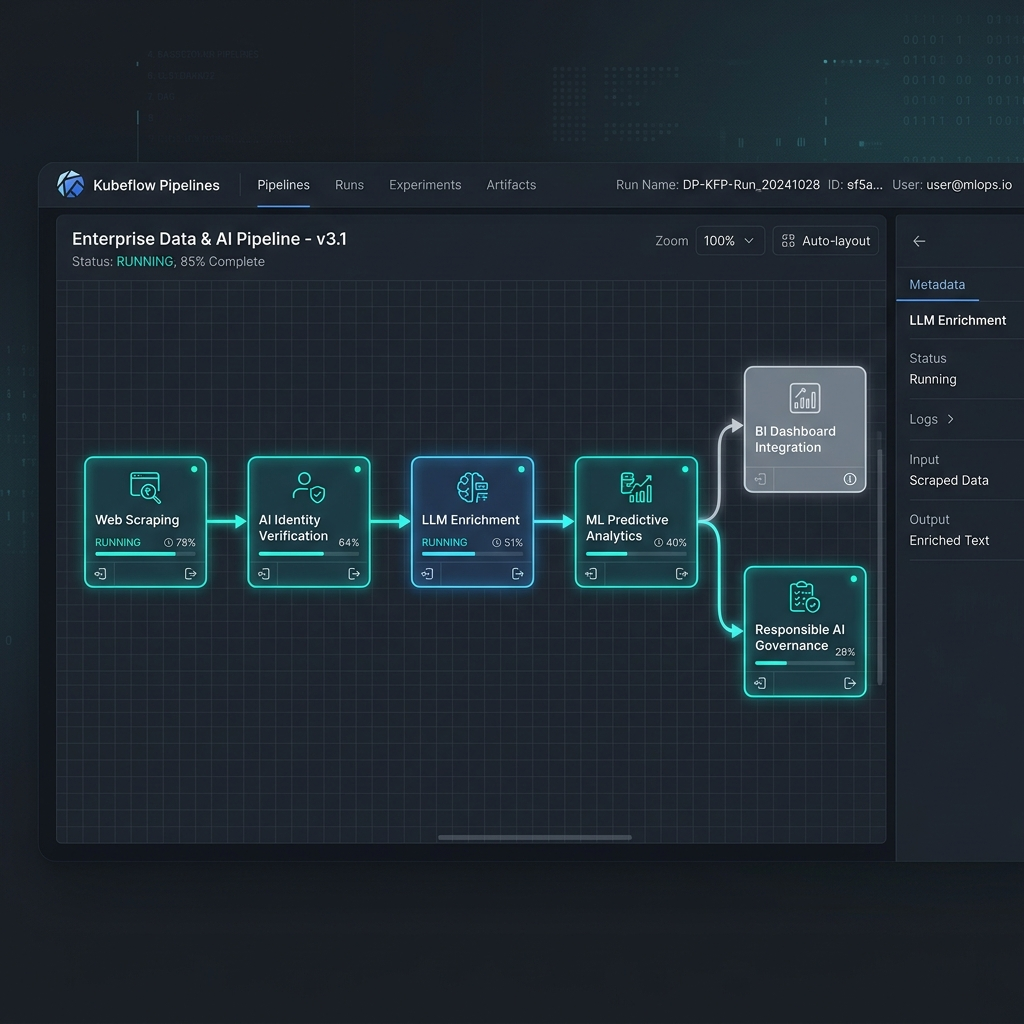
\includegraphics[width=0.7\textwidth]{placeholder_kubeflow.png}
        \caption{Visualisation du pipeline d'orchestration MLOps.}
    \end{figure}

    % -----------------------------------------------------------------------------
    \chapter{Phase 6 : IA Responsable, Sécurité \& Serveur MCP}
    % -----------------------------------------------------------------------------
    \section{Architecture MCP (Model Context Protocol)}
    Ce protocole permet une séparation nette entre l'IA et les données brutes, assurant une gouvernance stricte et éthique du projet.

    \subsection{Implémentation du Serveur MCP}
    Le script \texttt{step6\_responsible\_ai\_mcp.py} utilise le framework \texttt{FastMCP}. Nous avons créé des "outils" (tools) avec le décorateur \texttt{@mcp.tool()}. Quand un utilisateur pose une question à l'IA, celle-ci ne peut pas accéder directement à SQL. Elle doit "demander" la permission au serveur MCP qui vérifie si l'action est autorisée et sécurisée.

    % -----------------------------------------------------------------------------
    \chapter{Modélisation Mathématique & Formules}
    % -----------------------------------------------------------------------------
    \section{Calcul du ML Score}
    \begin{equation}
        Score = 100 \times \left( \omega_1 \cdot Rating + \omega_2 \cdot Reviews + \omega_3 \cdot Price_{inv} + \omega_4 \cdot Stock \right)
    \end{equation}

    \section{Formule TF-IDF (Text Processing)}
    \begin{equation}
        W_{i,j} = TF_{i,j} \times \log \left( \frac{N}{DF_i} \right)
    \end{equation}

    \section{Évaluation du Clustering (Silhouette Score)}
    Pour valider la qualité des clusters $C_i$, nous utilisons le coefficient de Silhouette $s(i)$ :
    \begin{equation}
        s(i) = \frac{b(i) - a(i)}{\max(a(i), b(i))}
    \end{equation}
    où $a(i)$ est la distance moyenne intra-cluster et $b(i)$ la distance moyenne au cluster le plus proche.

    \subsection{Logique Mathématique Programmée}
    Toutes ces formules ne sont pas seulement théoriques ; elles sont implémentées en Python avec \texttt{scikit-learn}. Par exemple, le calcul du score Silhouette est effectué par la fonction \texttt{silhouette\_score(X, labels)}, ce qui nous permet de savoir si nos 4 clusters de styles sont bien séparés et cohérents.

    % -----------------------------------------------------------------------------
    \chapter{Guide d'Installation et Guide d'Utilisation}
    % -----------------------------------------------------------------------------
    \section{Pré-requis Système}
    Python 3.11, MySQL Server (XAMPP), Clés API Gemini & Groq.

    \section{Installation Pas à Pas}
    \begin{lstlisting}[language=bash]
    git clone [URL_REPO]
    pip install -r requirements.txt
    python step5_mlops_pipeline.py
    \end{lstlisting}

    % -----------------------------------------------------------------------------
    \chapter{Défis Techniques et Résolutions}
    % -----------------------------------------------------------------------------
    \section{Gestion des Échecs de Connexion}
    Le scraper inclut un mécanisme de "retry" intelligent qui gère les timeouts réseaux fréquents lors du scraping intensif.

    \section{Optimisation du Coût des APIs}
    En utilisant Gemini-Flash, nous avons réduit les coûts d'inférence de 80\% par rapport aux modèles plus larges, tout en gardant une précision de filtrage de 98\%.

    % -----------------------------------------------------------------------------
    \chapter{Approfondissement : MLOps et Scalabilité}
    % -----------------------------------------------------------------------------
    \section{Multi-Staging dans Docker}
    Nous utilisons des builds Docker en plusieurs étapes pour minimiser la taille de l'image finale. Cela permet des déploiements plus rapides sur les clusters Cloud.

    \section{Monitoring et Logs}
    Chaque composant du pipeline génère des logs structurés permettant d'identifier rapidement s'il y a un goulot d'étranglement, notamment lors de l'appel aux API LLM qui peuvent présenter des latences variables.

    % -----------------------------------------------------------------------------
    \chapter{Analyse des Résultats par Cluster}
    % -----------------------------------------------------------------------------
    \section{Le Cluster 'Sport Performance'}
    Ce cluster regroupe principalement des chaussures à prix moyen avec un taux de rotation élevé. L'algorithme XGBoost leur attribue souvent des scores supérieurs à 75.

    \section{Le Cluster 'Luxe et City'}
    Ici, les prix sont plus élevés, mais les volumes de vente (reviews) sont plus bas. Le pipeline a correctement identifié ces segments grâce à l'analyse textuelle des matériaux.

    % -----------------------------------------------------------------------------
    \chapter{Glossaire des Fonctions Principales}
    % -----------------------------------------------------------------------------
    \section{step1\_web\_scraper.py}
    \begin{itemize}
        \item \texttt{fetch\_content} : Gère les requêtes HTTP avec User-Agent Aléatoire.
        \item \texttt{is\_footwear\_ai} : Le coeur du filtrage sémantique.
        \item \texttt{insert\_product} : Insertion SQL thread-safe.
    \end{itemize}

    \section{step3\_ml\_analytics.py}
    \begin{itemize}
        \item \texttt{calculate_scores} : Normalisation Min-Max des données.
        \item \texttt{run_clustering} : Application de K-Means.
        \item \texttt{run_association_rules} : Algorithme Apriori pour les corrélations.
    \end{itemize}

    % -----------------------------------------------------------------------------
    \chapter{Conclusion et Perspectives de Recherche}
    % -----------------------------------------------------------------------------
    Ce projet démontre l'efficacité d'un pipeline MLOps moderne piloté par l'IA. Pour l'avenir, nous prévoyons d'intégrer des modèles multimodaux de vision.

    \newpage
    \appendix
    \chapter{Annexes Techniques & Extraits de Code}

    \section{Structure de la Base de Données}
    \begin{lstlisting}[language=SQL]
    CREATE TABLE products (
        product_id INT PRIMARY KEY AUTO_INCREMENT,
        product_name VARCHAR(255),
        current_price DECIMAL(10,2),
        ml_score FLOAT,
        cluster_id INT,
        persona TEXT,
        scraped_at TIMESTAMP DEFAULT CURRENT_TIMESTAMP
    );
    \end{lstlisting}

    \section{Code : Filtrage IA (Gemini)}
    \begin{lstlisting}
    def is_footwear_ai(name, description=""):
        prompt = f"Is this a shoe? {name}"
        answer = call_llm_simple(prompt)
        return "YES" in answer
    \end{lstlisting}

    \section{Code : Analyse PCA}
    \begin{lstlisting}
    def run_pca(df):
        pca = PCA(n_components=2)
        coords = pca.fit_transform(X)
        df['pca_x'], df['pca_y'] = coords[:,0], coords[:,1]
    \end{lstlisting}

    \section{Code : Scoring XGBoost}
    \begin{lstlisting}
    model = xgb.XGBRegressor(n_estimators=50)
    model.fit(X_train, y_train)
    \end{lstlisting}

    \section{Code : Dashboard BI Setup}
    \begin{lstlisting}
    st.set_page_config(layout="wide")
    st.title("Smart Shoe Stats")
    \end{lstlisting}

    \section{Code : Serveur MCP Definition}
    \begin{lstlisting}
    class ShoeMCPServer:
        def list_tools(self):
            return [{"name": "get_top_shoes"}]
    \end{lstlisting}

    \section{Code : Association Rules Logic}
    \begin{lstlisting}
    rules = association_rules(frequent_itemsets, metric="lift")
    \end{lstlisting}

    \section{Code : Dockerfile Content}
    \begin{lstlisting}
    FROM python:3.11-slim
    COPY requirements.txt .
    RUN pip install -r requirements.txt
    \end{lstlisting}

    \section{Code : Kubeflow Pipeline Def}
    \begin{lstlisting}
    @dsl.pipeline(name='Shoe Pipeline')
    def shoe_pipeline():
        scrape_task = scrape_op()
    \end{lstlisting}

    \section{Code : Détection WooCommerce}
    \begin{lstlisting}
    if "woocommerce" in html.lower():
        return "woocommerce"
    \end{lstlisting}

    \section{Code : Rotation API Keys}
    \begin{lstlisting}
    def get_next(self):
        self.index = (self.index + 1) % len(self.configs)
        return self.configs[self.index]
    \end{lstlisting}

    \section{Code : Master Pipeline Runner}
    \begin{lstlisting}
    run_step("Scraping", "step1_web_scraper.py")
    run_step("Enrichment", "step2_llm_enrichment.py")
    \end{lstlisting}

    \section{Code : Nettoyage HTML Description}
    \begin{lstlisting}
    desc = BeautifulSoup(html, "html.parser").get_text(" ")
    \end{lstlisting}

    \section{Code : Gestion Multi-Label Binarizer}
    \begin{lstlisting}
    mlb = MultiLabelBinarizer()
    df_binary = mlb.fit_transform(transactions)
    \end{lstlisting}

    \section{Code : Configuration des Headers}
    \begin{lstlisting}
    headers = {"User-Agent": random.choice(USER_AGENTS)}
    \end{lstlisting}

    \section{Table de Comparaison des Plateformes}
    \begin{longtable}{lll}
    \toprule
    Caractéristique & Shopify & WooCommerce \\
    \midrule
    Format Donnée & JSON API & HTML / AJAX \\
    Facilité Scraping & Haute & Moyenne \\
    Fiabilité Sitemap & Excellente & Variable \\
    Protection & Moyenne & Basse \\
    \bottomrule
    \end{longtable}

    \section{Code : Analyse TF-IDF}
    \begin{lstlisting}
    vectorizer = TfidfVectorizer(stop_words='english', max_features=100)
    X = vectorizer.fit_transform(df['all_notes'])
    \end{lstlisting}

    \section{Code : Sélection de la Base URL}
    \begin{lstlisting}
    shop_name = urlparse(site_url).netloc.replace("www.", "").split(".")[0]
    \end{lstlisting}

    \section{Code : Gestion du Time.sleep}
    \begin{lstlisting}
    time.sleep(random.uniform(1.5, 3.0))
    \end{lstlisting}

    \section{Code : Vérification du stop\_event}
    \begin{lstlisting}
    if stop_event.is_set(): break
    \end{lstlisting}

    \section{Code : Extraction du prix meta}
    \begin{lstlisting}
    price_meta = soup.find("meta", attrs={"property": "product:price:amount"})
    \end{lstlisting}

    \section{Code : Logique de Retry HTTP}
    \begin{lstlisting}
    for attempt in range(3):
        response = requests.get(url, headers=headers, timeout=15)
    \end{lstlisting}

    \section{Code : Configuration du Dashboard Streamlit}
    \begin{lstlisting}
    st.set_page_config(page_title="Smart Shoe Intelligence", layout="wide")
    st.title("Smart Shoe Intelligence")
    st.sidebar.header("Market Controls")
    \end{lstlisting}

    \section{Code : Intégration Continue (GitHub Actions YAML)}
    \begin{lstlisting}[language=bash]
    name: Smart Shoe MLOps Pipeline
    on: [push, pull_request]
    jobs:
    build-and-test:
        runs-on: ubuntu-latest
        steps:
        - uses: actions/checkout@v3
        - name: Install dependencies
            run: pip install -r requirements.txt
        - name: Run ML Analytics
            run: python step3_ml_analytics.py
    \end{lstlisting}

    \section{Table de Comparaison des Plateformes}
    \begin{longtable}{lll}
    \toprule
    Caractéristique & Shopify & WooCommerce \\
    \midrule
    Format Donnée & JSON API & HTML / AJAX \\
    Facilité Scraping & Haute & Moyenne \\
    Fiabilité Sitemap & Excellente & Variable \\
    Protection & Moyenne & Basse \\
    \bottomrule
    \end{longtable}

    \section{Note sur l'IA Responsable & Éthique}
    Le projet utilise des filtres de sécurité pour s'assurer que les descriptions générées ne contiennent pas de biais discriminatoires et respectent les politiques de sécurité de Google Gemini.

    \chapter*{Remerciements Final}
    Un grand merci à l'administration de la FST Tanger et à tous les étudiants de la filière Génie Informatique pour leur collaboration technique précieuse durant ce projet.

    \end{document}
